\documentclass[tikz,border=3pt]{standalone}
\usepackage{amsmath}
\usepackage{tikz}
\usetikzlibrary{shapes.geometric,arrows.meta,patterns,calc}

\begin{document}
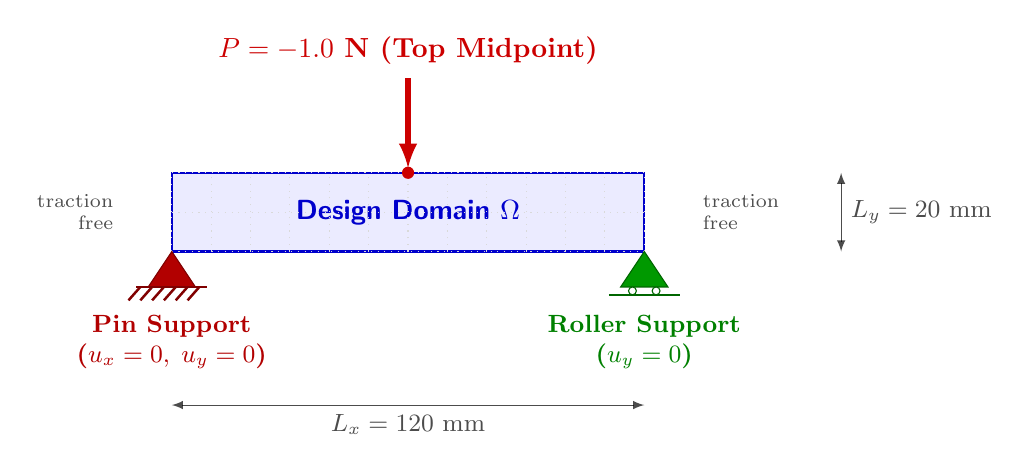
\begin{tikzpicture}[scale=1.0, >=latex]
  % FullMBBBeam2d: 120 x 20 mm, 绘图比例 0.05 -> 6.0 x 1.0
  % Design Domain
  \draw[thick, fill=blue!8, draw=blue!80!black] (0,0) rectangle (6,1);
  \node[font=\bfseries\sffamily, color=blue!80!black] at (3,0.5) {Design Domain $\Omega$};

  % Grid overlay
  \draw[step=0.5, gray!30, dotted] (0,0) grid (6,1);

  % Pin Support at Bottom Left (0, 0): u_x = u_y = 0
  \draw[fill=red!70!black, draw=red!50!black] (0,0) -- (-0.3,-0.45) -- (0.3,-0.45) -- cycle;
  \draw[thick, red!50!black] (-0.45,-0.45) -- (0.45,-0.45);
  \foreach \i in {-0.4,-0.25,-0.1,0.05,0.2,0.35} {
    \draw[line width=0.9pt, red!50!black] (\i,-0.45) -- (\i-0.15,-0.62);
  }
  \node[below, red!70!black, font=\small\bfseries, align=center] at (0,-0.68)
    {Pin Support\\($u_x = 0,\; u_y = 0$)};

  % Roller Support at Bottom Right (120, 0): u_y = 0
  \draw[fill=green!60!black, draw=green!40!black] (6,0) -- (5.7,-0.45) -- (6.3,-0.45) -- cycle;
  \draw[thick, green!40!black] (5.55,-0.55) -- (6.45,-0.55);
  \draw[fill=white, draw=green!40!black] (5.85,-0.5) circle (0.05);
  \draw[fill=white, draw=green!40!black] (6.15,-0.5) circle (0.05);
  \node[below, green!50!black, font=\small\bfseries, align=center] at (6,-0.68)
    {Roller Support\\($u_y = 0$)};

  % Concentrated Point Load at Top Midpoint (60, 20)
  \fill[red!80!black] (3,1) circle (2.2pt);
  \draw[->, ultra thick, red!80!black, line width=2pt] (3,2.2) -- (3,1.06);
  \node[above, red!80!black, font=\bfseries] at (3,2.25) {$P = -1.0\text{ N}$ (Top Midpoint)};

  % Traction-free remainder of the boundary
  \node[left, gray!60!black, font=\scriptsize, align=right] at (-0.62,0.5) {traction\\free};
  \node[right, gray!60!black, font=\scriptsize, align=left] at (6.62,0.5) {traction\\free};

  % Dimensions
  \draw[<->, opacity=0.7] (0,-1.95) -- (6,-1.95) node[midway, below, font=\small] {$L_x = 120\text{ mm}$};
  \draw[<->, opacity=0.7] (8.5,0) -- (8.5,1) node[midway, right, font=\small] {$L_y = 20\text{ mm}$};
\end{tikzpicture}
\end{document}
